\documentclass{article}

\usepackage[margin=1in]{geometry}
\usepackage{color}
\usepackage{hyperref}
\usepackage{soul}
\usepackage{float}
\usepackage{amsmath}

\usepackage[sc]{mathpazo}
\linespread{1.20}         % Palatino needs more leading (space between lines)
\usepackage[T1]{fontenc}
\usepackage{microtype}
\usepackage{listings}
\usepackage{courier}
\usepackage{graphicx}

\definecolor{mygreen}{rgb}{0,0.6,0}
\definecolor{light-gray}{gray}{0.95}

\lstset{basicstyle=\footnotesize\ttfamily,breaklines=true,language=Prolog}
\lstset{frame=single,commentstyle=\color{mygreen}}
\lstset{aboveskip=0.5cm,belowskip=0.3cm}
\lstset{backgroundcolor=\color{light-gray}}

\hypersetup{pdfpagemode=UseNone}

\newcommand{\manager}{\texttt{manager} }
\newcommand{\eagent}{\texttt{elevator agent} }
\newcommand{\eagents}{\texttt{elevator agents} }
\newcommand{\todo}[1] {\hl{TODO: #1}}
\newcommand{\horrule}[1]{\rule{\linewidth}{#1}}
\setlength{\parindent}{0cm}

\title{ 	
		\usefont{OT1}{bch}{b}{n}
		\normalfont \normalsize \textsc{Delft University of Technology \protect\\ Data Visualization 2015-2016} \\ [25pt]
		\horrule{0.5pt} \\[0.4cm]
		\huge Football Match Visualization Project \\
		\horrule{2pt} \\[0.5cm]
}
\author{
		\normalfont 								\normalsize
        Afentoulidis Grigorios 4521862\\[-3pt]		\normalsize
        \today
}
\date{}
\begin{document}
\lstset{language=Prolog}
\maketitle

\section{Individual Report}
My work on the project is focused on the graphs that we developed and i will present in the next sections. I also authored a python script that extracted the data we needed form the initial data set.


\subsection{Radar Chart}
For the radar chart i used Chart.js. I collected the statistics data of the match from the internet and i coded and added the radar chart to our web page. I have chosen statistics that are related with accuracy so that they can be expressed as percentages and thus be comparable. I have also opted for color hues that would be easily distinguishable and an opacity that would allow the areas of the plot to overlap without creating new colors and distorting the information of the chart. The chart plot has also embedded interactivity in order to show the values of the statistics when the mouse of the user is hovering over the different areas of the chart. A figure of this chart is shown below.

\begin{figure}[ht!]
\centering
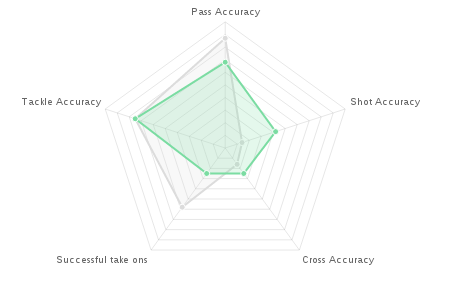
\includegraphics[scale=0.35]{radar}
\end{figure}

\subsection{Bar Chart}
Another visualization that i worked on is that of the distance of a player to all others in the current time. This is visualized by a bar chart that is related to a click events made in the field visualizations (2d and 3d). Whenever a player is picked the bar chart adapts to that selection automatically and animates the distances to all other players as the time passes by. When stop is pressed the bar chart will show the current time distances and is available for inspection of the values by the user. This chart was also developed in Chart.js and is depicted below.

\begin{figure}[ht!]
\centering
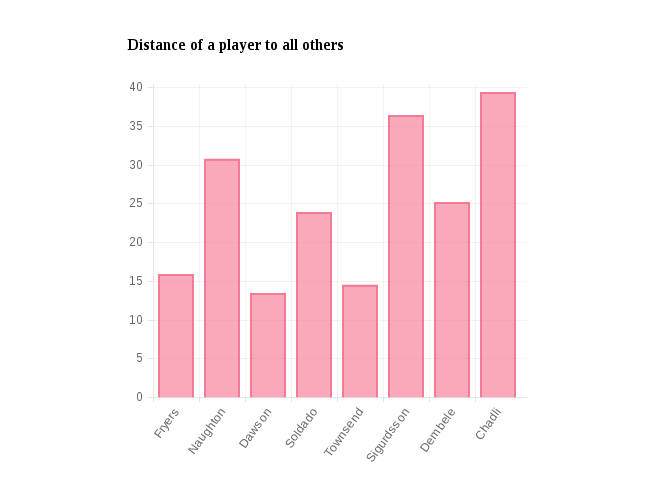
\includegraphics[scale=0.35]{bar}
\end{figure}

\subsection{Line Graphs}
The line graphs are visualizations that are highlighting player specific statistics for the whole game when a player is selected by the field visualizations. Those statistics are related to energy, speed and total distance covered for every minute. The user has the option of selecting which metric he wants to visualize and see per minute the values related to this. I also implemented a focus effect on the visualization that gives the values (minute and metric) when a user hovers over the graph. A picture of a speed graph is shown below.

\begin{figure}[ht!]
\centering
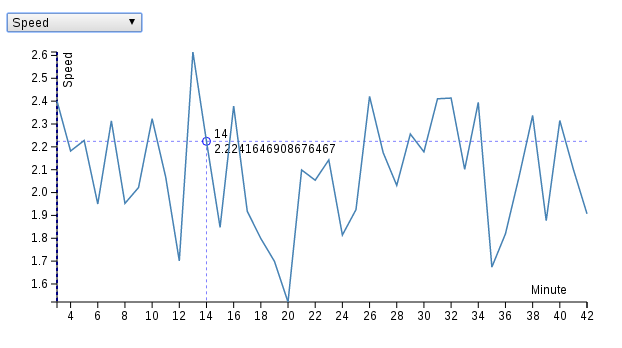
\includegraphics[scale=0.35]{line}
\end{figure}
 

\bibliographystyle{ieeetr}
\bibliography{report_group23}
\end{document}